\documentclass[letterpaper]{article} % DO NOT CHANGE THIS
\usepackage[submission]{aaai2027}  % DO NOT CHANGE THIS
% The serif, sans-serif, and monospaced fonts are loaded automatically by
% aaai2027.sty (newtxtext, helvet, courier). DO NOT add \usepackage{times},
% \usepackage{helvet}, \usepackage{courier}, or any other font package.
\usepackage[hyphens]{url}  % DO NOT CHANGE THIS
\usepackage{graphicx} % DO NOT CHANGE THIS
\urlstyle{rm} % DO NOT CHANGE THIS
\def\UrlFont{\rm}  % DO NOT CHANGE THIS
\usepackage{natbib}  % DO NOT CHANGE THIS AND DO NOT ADD ANY OPTIONS TO IT
\usepackage{caption} % DO NOT CHANGE THIS AND DO NOT ADD ANY OPTIONS TO IT
\frenchspacing  % DO NOT CHANGE THIS
%
% These are recommended to typeset algorithms but not required. See the subsubsection on algorithms. Remove them if you don't have algorithms in your paper.
\usepackage{algorithm}
% \usepackage{algorithmic}  % superseded by algorithmicx +
% algpseudocode below, which this preamble's \algnewcommand needs;
% loading both makes \algorithmic doubly defined.

\newcommand{\eg}{{\textit{e.g.}}}
\newcommand{\ie}{{\textit{i.e.}}}
\newcommand{\etal}{{\textit{et al.}}}
\newcommand\TODO[1]{{\color{red} TODO: {#1}}}
\usepackage{algorithmicx}
\usepackage{amsmath}
% \usepackage{algorithm2e}
\algnewcommand{\LeftComment}[1]{\Statex \(\triangleright\) #1}
% \usepackage{import}
% \usepackage{lipsum}
\usepackage{threeparttable}
\usepackage{algpseudocode}
\usepackage{booktabs}
\usepackage{multirow}
\usepackage{rotating}

\newcommand{\zimeng}[1]{\textcolor{teal}{{\it [Zimeng: #1]}}}

%
% These are recommended to typeset listings but not required. See the subsubsection on listing. Remove this block if you don't have listings in your paper.
\usepackage{amsmath}
\usepackage{listings}
\DeclareCaptionStyle{ruled}{labelfont=normalfont,labelsep=colon,strut=off} % DO NOT CHANGE THIS
\lstset{%
	basicstyle={\footnotesize\ttfamily},% footnotesize acceptable for monospace
	numbers=left,numberstyle=\footnotesize,xleftmargin=2em,% show line numbers, remove this entire line if you don't want the numbers.
	aboveskip=0pt,belowskip=0pt,%
	showstringspaces=false,tabsize=2,breaklines=true}
\floatstyle{ruled}
\newfloat{listing}{tb}{lst}{}
\floatname{listing}{Listing}

%
% Recommended for better-looking tables
\usepackage{booktabs}

%
% Keep the \pdfinfo as shown here. There's no need
% for you to add the /Title and /Author tags.
\pdfinfo{
/TemplateVersion (2027.1)
}

% DISALLOWED PACKAGES
% \usepackage{authblk} -- This package is specifically forbidden
% \usepackage{balance} -- This package is specifically forbidden
% \usepackage{CJK} -- This package is specifically forbidden
% \usepackage{float} -- This package is specifically forbidden
% \usepackage{flushend} -- This package is specifically forbidden
% \usepackage{fullpage} -- This package is specifically forbidden
% \usepackage{geometry} -- This package is specifically forbidden
% \usepackage{hyperref} -- This package is specifically forbidden
% \usepackage{navigator} -- This package is specifically forbidden
% (or any other package that embeds links such as navigator or hyperref)
% \usepackage{indentfirst} -- This package is specifically forbidden
% \usepackage{layout} -- This package is specifically forbidden
% \usepackage{multicol} -- This package is specifically forbidden
% \usepackage{nameref} -- This package is specifically forbidden
% \usepackage{savetrees} -- This package is specifically forbidden
% \usepackage{setspace} -- This package is specifically forbidden
% \usepackage{stfloats} -- This package is specifically forbidden
% \usepackage{tabu} -- This package is specifically forbidden
% \usepackage{titlesec} -- This package is specifically forbidden
% \usepackage{tocbibind} -- This package is specifically forbidden
% \usepackage{ulem} -- This package is specifically forbidden
% \usepackage{wrapfig} -- This package is specifically forbidden
% DISALLOWED COMMANDS
% \nocopyright -- Your paper will not be published if you use this command
% \addtolength -- This command may not be used
% \balance -- This command may not be used
% \baselinestretch -- Your paper will not be published if you use this command
% \clearpage -- No page breaks of any kind may be used for the final version of your paper
% \columnsep -- This command may not be used
% \newpage -- No page breaks of any kind may be used for the final version of your paper
% \pagebreak -- No page breaks of any kind may be used for the final version of your paper
% \pagestyle -- This command may not be used
% \tiny -- This is not an acceptable font size.
% \vspace{- -- No negative value may be used in proximity of a caption, figure, table, section, subsection, subsubsection, or reference
% \vskip{- -- No negative value may be used to alter spacing above or below a caption, figure, table, section, subsection, subsubsection, or reference

\setcounter{secnumdepth}{0} %May be changed to 1 or 2 if section numbers are desired.

% The file aaai2027.sty is the style file for AAAI Press
% proceedings, working notes, and technical reports.
%

% Title

% Your title must be in mixed case, not sentence case.
% That means all verbs (including short verbs like be, is, using,and go),
% nouns, adverbs, adjectives should be capitalized, including both words in hyphenated terms, while
% articles, conjunctions, and prepositions are lower case unless they
% directly follow a colon or long dash
\title{AAAI Press Anonymous Submission\\Instructions for Authors Using \LaTeX{}}
\author{
    %Authors
    % All authors must be in the same font size and format.
    Written by AAAI Press Staff\textsuperscript{\rm 1}\thanks{With help from the AAAI Publications Committee.}\\
    AAAI Style Contributions by Peter Patel Schneider,
    Sunil Issar,\\
    J. Scott Penberthy,
    George Ferguson,
    Hans Guesgen,
    Francisco Cruz\equalcontrib\corresponding,
    Marc Pujol-Gonzalez\equalcontrib\corresponding
}
\affiliations{
    %Afiliations
    \textsuperscript{\rm 1}Association for the Advancement of Artificial Intelligence\\
    % If you have multiple authors and multiple affiliations
    % use superscripts in text and roman font to identify them.
    % For example,

    % Sunil Issar\textsuperscript{\rm 2},
    % J. Scott Penberthy\textsuperscript{\rm 3},
    % George Ferguson\textsuperscript{\rm 4}\corresponding,
    % Hans Guesgen\textsuperscript{\rm 5}
    % Note that the comma should be placed after the superscript

    1101 Pennsylvania Ave, NW Suite 300\\
    Washington, DC 20004 USA\\
    % email address must be in roman text type, not monospace or sans serif
    proceedings-questions@aaai.org
%
% See more examples next
}

%Example, Single Author, ->> remove \iffalse,\fi and place them surrounding AAAI title to use it
\iffalse
\title{My Publication Title --- Single Author}
\author {
    Author Name
}
\affiliations{
    Affiliation\\
    Affiliation Line 2\\
    name@example.com
}
\fi

\iffalse
%Example, Multiple Authors, ->> remove \iffalse,\fi and place them surrounding AAAI title to use it
\title{My Publication Title --- Multiple Authors}
\author {
    % Authors
    First Author Name\textsuperscript{\rm 1,\rm 2}\equalcontrib,
    Second Author Name\textsuperscript{\rm 2}\equalcontrib,
    Third Author Name\textsuperscript{\rm 1}\corresponding
}
\affiliations {
    % Affiliations
    \textsuperscript{\rm 1}Affiliation 1\\
    \textsuperscript{\rm 2}Affiliation 2\\
    firstAuthor@affiliation1.com, secondAuthor@affilation2.com, thirdAuthor@affiliation1.com
}
\fi


\begin{document}

\maketitle

\begin{abstract}
AAAI creates proceedings, working notes, and technical reports directly from electronic source furnished by the authors. To ensure that all papers in the publication have a uniform appearance, authors must adhere to the following instructions.
\end{abstract}

% Uncomment the following to link to your code, datasets, an extended version or similar.
% You must keep this block between (not within) the abstract and the main body of the paper.
% Make sure that you do not de-anonymize yourself with these links.
% \begin{links}
%     \link{Code}{https://aaai.org/example/code}
%     \link{Datasets}{https://aaai.org/example/datasets}
%     \link{Extended version}{https://aaai.org/example/extended-version}
% \end{links}

\input{01-Introduction}
\input{02-RelatedWork}
\section{Method}
\label{sec:method}

This section summarises the ONE-NAS algorithm \cite{lyu2023onenas},
defines the two prediction rules compared in this study, and describes
the deployment architecture in which search and inference are executed
on separate hardware. Configuration values are deferred to
Section~\ref{sec:setup}.

\subsection{Online Neuroevolution}

ONE-NAS maintains a population of RNNs and evolves both their
architectures and their weights as data arrive. Each individual, termed
a genome, is a directed graph in which hidden nodes are instantiated
from a library of recurrent cell types. Evolution begins from a minimal
genome containing only input-to-output connections. Offspring are
produced by mutation (insertion or deletion of nodes and edges,
insertion of recurrent edges, and change of cell type) and by crossover
between two parents. Weights are inherited from the parent for every
retained component and randomly initialised only for newly introduced
components. This Lamarckian inheritance reduces the training required
per offspring to a small number of backpropagation epochs and is a
prerequisite for operating within the data cadence.

The population is partitioned into $N$ islands. Each island maintains an
elite set of fixed size, generates a fixed number of offspring per
generation from that set, and admits genetic material from other
islands only through inter-island crossover at a low rate. Islands
consequently converge to distinct regions of the architecture space. To
counteract stagnation, at a fixed interval the island whose best elite
has the worst fitness is cleared and re-initialised from the global
best genome.

\subsection{Online Protocol}

The input stream is partitioned into windows of fixed length in trading
days, and one generation is executed per window. Let $\mathcal{H}_t$
denote the history available at generation $t$. In generation $t$, each
island generates offspring from its elites; offspring are trained on
worker processes using subsequences sampled from $\mathcal{H}_t$; all
genomes, elite and offspring, are evaluated by mean squared error on
the most recent windows of $\mathcal{H}_t$, which are excluded from
training; and each island retains the top-ranked genomes as its elite
set. The window revealed during generation $t$ is then appended to form
$\mathcal{H}_{t+1}$. Because fitness is measured on recent data while
training draws on the full history, the population tracks the current
regime without discarding earlier ones. Genome generation is performed
by a single master process and training is distributed asynchronously
across workers, so that the wall-clock cost of a generation is governed
by the number of workers rather than the population size.

\subsection{Prediction Rules}
\label{sec:prediction_rules}

At the end of generation $t$, the algorithm exposes the elite set of
each island and the genome of best fitness across all islands. The
selection of genomes used to predict window $t{+}1$ is a scoring-time
decision that does not affect the search. Two rules are compared.

Under the \emph{single champion} rule, the global best genome alone
produces the prediction. This is the rule used in all prior ONE-NAS
work.

Under the \emph{island-champion ensemble} rule, the best elite of each
island produces a prediction, giving $N$ predicted cross-sections. Each
is converted to ranks, and the ranks are averaged across members. Rank
aggregation is used in place of output averaging because the members
are independently trained networks with non-comparable output scales,
and because every trading rule considered here depends only on the
ordering of the prediction.

Both rules are evaluated on the same runs. Any difference between them
is therefore attributable to the use of the evolved population rather
than to its construction.

\subsection{Deployment Architecture}
\label{sec:deployment}

Search and inference are executed on separate machines, reflecting the
asymmetry in their computational requirements: population training is
parallel and expensive, whereas evaluating the resulting networks is
not. Figure~\ref{fig:deployment} depicts the pipeline.

\paragraph{Search host.} ONE-NAS is executed on a cloud instance or a
workstation with sufficient cores to train a generation's offspring in
parallel, using one master process and a pool of training workers. The
host stores the price history, advances the window clock, and performs
all evolutionary operations.

\paragraph{Endpoint.} Inference is performed on a Raspberry Pi,
selected as a deliberately constrained target with substantially less
compute and memory than a typical consumer laptop or office desktop.
Demonstrating that inference meets the data cadence on this device
establishes a lower bound on the hardware required at the point of use.
The endpoint stores only the most recently received genomes and the
current day's feature vectors; no training is performed on the device.

\paragraph{Model hand-off.} Transfer of genomes from host to endpoint is
a step of every generation. Upon completion of selection in generation
$t$, the master serialises the genomes designated to predict window
$t{+}1$ (the global best genome, or the $N$ island champions, according
to the prediction rule) into a binary encoding of graph structure, cell
types, and weights, and transmits the file to the endpoint over TCP/IP.
The endpoint deserialises the networks and produces a prediction for
each day of window $t{+}1$ as its features become available, applying
the rank aggregation of Section~\ref{sec:prediction_rules} when an
ensemble is received. Concurrently, the host generates and trains
generation $t{+}1$. Prediction and search thus overlap in time, as in
the original ONE-NAS design, but are decoupled across hardware.

Two properties of this architecture are relevant to deployment. First,
inference cost scales only with $N$ and the number of securities, so
increasing the island count does not alter the endpoint's hardware
requirement. Second, the endpoint is stateless with respect to the
search: in the event of host unavailability, it continues to predict
with the most recently received genomes and resumes upon the next
hand-off.
% 04-Dataset.tex -- data construction and experimental setup.
%
% AAAI COMPLIANCE: no added packages, and none of the commands aaai2027
% forbids (no \setlength, \vspace, \vskip, \newpage, \tiny, ...). Column
% padding is trimmed with @{} rather than by resetting \tabcolsep.
%
% SCOPE: experimental detail only -- what was run, on what data, scored
% how. No findings, no interpretation; those live in the Results section.
%
% \text comes from amsmath, which this template does not load; the
% fallback keeps the file self-contained if any \text survives an edit.
% It is a no-op when amsmath is present.
\providecommand{\text}[1]{\mathrm{#1}}

\section{Data}

\subsection{Universe and Source}

All data are daily CRSP records for U.S.\ common equities. From the
mid-- and upper-mid-capitalisation segment we form four disjoint panels,
denoted $V1$--$V4$, of 50 tickers each; the four share no constituents,
so 200 distinct names are used in total. Each panel is stored as one CSV
per ticker plus a panel-level date index carrying the aligned raw price
and transaction-cost columns for every name.

Every panel ends on 2024-12-31 but they begin on different dates,
because a panel starts only once all 50 of its constituents have priced
history: $V1$ runs from 2004-08-16, $V2$ from 2004-12-17, $V3$ from
2004-10-27 and $V4$ from 2004-02-09, giving 5{,}130, 5{,}043, 5{,}079 and
5{,}257 trading days respectively. The differing lengths affect only the
burn-in each panel receives; the tuning and trading periods are the same
calendar spans for all four, so no arm gains or loses scored days.

Panel membership is fixed for the whole sample: a ticker is either in a
panel for its entire history or not in it at all. This removes
index-reconstitution effects from the comparison, at the cost of
conditioning the universe on names that survived to the end of the
sample. All methods trade the identical universe, so the conditioning
applies equally to every arm reported.

\subsection{Features and Prediction Target}

Each model sees seven per-stock features, all computed causally from
information available at or before the formation day:

\begin{itemize}\itemsep2pt
\item \texttt{RET} --- the raw daily return.
\item \texttt{RET\_CS\_IN} --- the cross-sectional rank-normal score of
      \texttt{RET} on the same day, i.e.\ $\Phi^{-1}\!\big((\mathrm{rank}_t(i)-0.5)/N\big)$
      over the $N$ names priced that day.
\item \texttt{BA\_SPREAD} --- the quoted bid--ask spread, the gap between
      the best buying and selling price, which proxies how costly the
      stock is to trade.
\item \texttt{ILLIQUIDITY} --- Amihud illiquidity: absolute return over
      dollar volume, smoothed over 21 days and logged. It is large when
      a small amount of trading moves the price a lot.
\item \texttt{REV21\_1} --- short-horizon reversal: the compounded return
      over the 20 days before the formation day, excluding it. Recent
      winners tend to give some of it back, so this is predictive with a
      negative sign.
\item \texttt{TURN\_RATIO} --- turnover acceleration: recent trading
      activity relative to its own longer-run level, as the mean of
      $\log(1+\mathrm{turnover})$ over the last 5 days minus the same
      mean over the last 63. It rises when a stock starts attracting
      unusual attention.
\item \texttt{VOL21} --- realised volatility, the standard deviation of
      \texttt{RET} over the trailing 21 days.
\end{itemize}

These are standard predictors in the empirical asset pricing literature
rather than novel ones; the contribution of this paper is in the
architecture search, so the feature set is deliberately conventional.

The last five of these are additionally mapped, per date, to their
cross-sectional rank on $[-1,1]$, so that no feature carries a level that
drifts across the two decades of the sample.

The prediction target is \texttt{RET\_CS}: the next day's return, rank-
normalised across the cross-section of that day by the same $\Phi^{-1}$
transform. Predicting a cross-sectional rank rather than a raw return
makes the target stationary by construction and matches how the
predictions are consumed --- every trading rule in this paper reads only
the ordering of the predicted cross-section.

Realised returns used for scoring are CRSP \texttt{RET}, which is adjusted
for splits and dividends. Prices and per-name transaction costs enter only
through the cost model below.

\section{Experimental Setup}

\subsection{Online Evaluation Protocol}

Every method is evaluated prequentially: on each scored day the model
predicts the next day's cross-section, the realised outcome is then
revealed, and the model updates. No model ever sees a label before
predicting it, and no model is refit on the scored span with hindsight.

ONE-NAS advances on a weekly clock. One generation corresponds to a
\texttt{window\_step} of 5 trading days; each genome is trained on
sequences of length $L=40$ and validated on the 5 most recent windows.
The number of training windows is set per panel so that the clock lands on
the intended calendar span --- 712, 695, 702 and 738 windows for
$V1$--$V4$ on the evaluation span, and 511, 493, 501 and 536 on the
tuning span.

The sample is divided into three disjoint spans, used for three distinct
purposes:

\begin{itemize}\itemsep2pt
\item \textbf{Burn-in}, through 2021-12-31. The population evolves online
      throughout, but nothing is traded or scored. A further 50 warm-up
      generations precede any recorded prediction, so the population that
      begins trading is mature rather than cold-started.
\item \textbf{Tuning}, 2016-01-01 to 2019-12-31. Every configuration
      decision --- hyperparameter screen, island count --- is made here,
      disjoint from the trading period.
\item \textbf{Trading}, 2022-01-01 to 2024-12-31. All reported results
      are on this period, which is also the period the prior study on
      these panels evaluated, so the two are directly comparable.
\end{itemize}

\subsection{Search Configuration and Prediction Rule}

The ONE-NAS settings are listed in Table~\ref{tab:hps} and were selected
on the tuning span. Node types available to the search are simple,
UGRNN, MGU, GRU, $\Delta$-RNN and LSTM recurrent cells.

A single run yields, at every generation, both the elite population of
each island and the single best genome overall, so the prediction rule is
a scoring-time choice rather than a property of the run. Two rules are
reported. The \emph{single champion} rule takes the global-best genome, as
in prior ONE-NAS work. The \emph{ensemble} rule takes one champion per
island --- the lowest-validation-error elite of each --- converts each
member's predicted cross-section to ranks, and averages the ranks. Rank
averaging is used rather than averaging predictions because the members
are separately trained networks whose output scales are not comparable.

\subsection{Hyperparameter Search}

Every configuration decision was made on the tuning span and is listed
here in full, so that the selected values in Table~\ref{tab:hps} can be
read against what was actually considered.

The search is single-axis around the registered control configuration:
each cell changes one setting and is compared against the control on
identical (panel, seed) cells. Sixteen configurations were trained ---
the control plus fifteen variants:

\begin{itemize}\itemsep2pt
\item \textbf{Fitness signal.} Selection on validation MSE (control),
      on cross-sectional rank IC, and on a gated rank IC.
\item \textbf{Prediction target.} 1-day cross-sectional rank-normal
      return (control) and the 5-day equivalent, the latter also in
      combination with gated-IC selection.
\item \textbf{Population structure.} Elite/generated ratios of 8/5
      (control), 5/10 and 5/15; repopulation every 25, 50 (control) and
      100 generations.
\item \textbf{Training budget.} 2000 (control) and 600 training
      subsequences per genome; 10 (control) and 20 backpropagation
      epochs per genome; one (control) and two generations per window.
\item \textbf{Replay sampling.} Prioritised replay at
      $\alpha \in \{0.4, 0.6\ (\text{control}), 0.8\}$, at
      $\lambda \in \{0.007\ (\text{control}), 0.021\}$, and uniform
      sampling with prioritisation disabled.
\item \textbf{Island count.} 8, 16, 20, 40, 50 and 60
      (Table~\ref{tab:tunewidth}).
\end{itemize}

Selection used the tuning-span rank IC as the primary objective with the
registered book's net return and Sharpe as an economic co-primary, and
required a paired improvement over the control to adopt a change. No
single-axis variant met that bar, so the control configuration is the one
reported; the island count is the one axis where a change was adopted,
and the value chosen sits on the plateau of Table~\ref{tab:tunewidth}
rather than at its nominal maximum. Table~\ref{tab:invariance} reports
every trained cell.

Several axes were deliberately not searched, having been settled by
earlier work on this data: sequence length, the number of validation
sets, the node-type library, window geometry, and the ensemble's width
and combination rule.

\subsection{Baselines}

Four online baselines trade the same books on the same panels under the
same costs. All are single networks; the reported cell is the mean over
independent runs, not the return of an ensemble of those runs.

\begin{itemize}\itemsep2pt
\item \textbf{Online LSTM} --- one LSTM, 8 hidden units, sequence length
      10, Adam at $10^{-3}$, one gradient step per trading day with a
      1000-day replay buffer.
\item \textbf{Online GRU} --- as above with a GRU cell and sequence
      length 5.
\item \textbf{Periodic LSTM} --- the same LSTM architecture refit from
      scratch each month for up to 4000 steps, rather than updated daily.
\item \textbf{Online AR} --- a first-order autoregression fitted by online
      gradient descent at $\eta=10^{-4}$. Deterministic, so it contributes
      one run per panel rather than one per seed.
\end{itemize}

All baselines predict the same cross-sectionally demeaned target as
ONE-NAS.

\subsection{Trading Books}

A \emph{book} is the rule that turns a day's predicted ranking into
actual positions, and it is what converts prediction quality into money.
All three books used here are \emph{long--short}: they buy (go
\emph{long}) the names predicted to do best and sell borrowed shares of
(go \emph{short}) the names predicted to do worst, in equal dollar
amounts. Equal amounts on each side make the book roughly
\emph{dollar-neutral}, so it profits from the top names outperforming the
bottom ones rather than from the market rising, and a rising or falling
market largely cancels out. This is why the books can be compared against
each other on skill rather than on market exposure, and why their returns
are not comparable to simply holding the market.

One registered primary construction is used, with two further
constructions reported as sensitivities.

The \textbf{sleeves} book is the registered primary: Jegadeesh--Titman
overlapping portfolios. Each day a new \emph{sleeve} --- one small
long--short portfolio --- goes long the top $k=10$ names and short the
bottom 10 by predicted rank, at $(\$100/H)/k$ per name per side with
holding period $H=10$ days; the sleeve formed $H$ days earlier is
retired. Ten sleeves are therefore live at once, each holding for ten
days, so the book turns over about a tenth of itself per day rather than
rebuilding daily. Costs are charged on the change in \emph{aggregate}
per-name position, so a name held by several sleeves at once is netted
rather than bought and sold repeatedly. Because only the ordering of each
day's predictions is read, every metric is invariant to any strictly
monotone transform of a model's outputs --- a model that doubles all its
predictions, or applies any order-preserving rescaling, trades
identically.

The \textbf{banded} book enters a name at predicted rank $\le 10$ and
holds it until its rank passes 35, following the buy/hold-spread
construction used to reduce turnover in the transaction-cost literature.
The \textbf{Algorithm 1} book is the conditional long--short rule of the
prior study, which rebalances only when all ten top predictions are
positive and all ten bottom predictions negative.

Books are funded with \$100 of capital and, when fully invested, hold
\$100 long and \$100 short, so \$200 of stock changes hands in total ---
the \emph{gross notional}.

Trading is not free, and the cost is charged explicitly. Every trade pays
the \emph{bid--ask spread}: the gap between what a buyer pays and a
seller receives, which is wide for thinly traded stocks and narrow for
liquid ones. We take that cost per name from the CRSP cost field and
apply it to the value actually traded, rather than assuming one flat rate
for every stock, so illiquid names are correctly penalised. All returns
reported in this paper are \emph{net}: costs have already been deducted.

\subsection{Metrics}

Two families are reported: how good the predictions are, and what the
resulting book earns.

\emph{Prediction quality} is the \textbf{rank IC} (information
coefficient): on each day, the Spearman rank correlation between the
predicted ordering of the cross-section and the realised one, averaged
over scored days. It is the natural accuracy measure here because the
books read only the ordering. Values are small by construction --- daily
cross-sectional return is mostly noise, and a rank IC of $0.01$--$0.02$
is a usable signal in this literature, not a weak one.

\emph{Economics} covers four quantities:

\begin{itemize}\itemsep2pt
\item \textbf{Net return}, the cumulative profit and loss over the period
      as a percentage of the starting \$100, after costs.
\item \textbf{Sharpe ratio}, the mean daily return divided by its
      standard deviation, annualised. It measures return per unit of
      volatility, so a strategy that earns the same amount more smoothly
      scores higher. Roughly, above 1 is good for a strategy of this
      kind.
\item \textbf{Maximum drawdown} (MDD), the largest peak-to-trough fall in
      cumulative profit over the period --- the worst loss an investor
      who entered at the worst moment would have sat through.
\item \textbf{Turnover}, mean daily traded value as a fraction of gross
      notional. A turnover of $0.12$ means about $12\%$ of the book is
      replaced each day; lower turnover means less exposure to
      transaction costs.
\end{itemize}

Finally, a return can look impressive merely by taking well-known risks,
so we check whether it survives that. Each arm's daily book return is
regressed on the four standard \emph{factors} of the empirical asset
pricing literature --- the market, firm size, value, and momentum
(Fama--French three-factor plus momentum). The slope on the market factor
is the \textbf{beta}, the portfolio's sensitivity to the market as a
whole: a beta near $1$ moves with the market, and one near $0$ is
insulated from it. The intercept is the \textbf{alpha}, the average
return left over once those four exposures are accounted for, and it is
alpha rather than raw return that indicates genuine skill. Standard
errors use the Newey--West correction at lag 10, which allows for daily
returns being autocorrelated rather than independent.

\subsection{Replication and Statistical Comparison}

The unit of replication is one (panel, seed) cell. Unless stated
otherwise, ONE-NAS arms comprise 10 seeds $\times$ 4 panels $=40$ cells.
The baselines were run at higher replication --- 48 seeds for online LSTM,
40 for online GRU and periodic LSTM --- and their own means are reported
at that full replication.

Comparisons between arms are paired within (panel, seed) cells, so that
panel and seed effects cancel, and the reported $t$ is a paired $t$ over
those cells. Where two arms do not share a seed set, the pairing is
restricted to the cells they have in common and $n$ is stated.

\subsection{Compute Environment}

All searches ran on ACCESS Anvil. Each run occupied one node of the
\texttt{wholenode} partition with 128 MPI ranks, one acting as the master
that maintains the island populations and distributes genomes, and the
remaining 127 as workers that train and evaluate them. The island count
is a search parameter and is independent of the rank count, so the worker
pool is identical across every configuration reported. Baselines are
single-process and were run on the same hardware.

\subsection{Pre-Registration}

The scored configuration, evaluation span, trading book and metrics were
committed to the repository before the evaluation span was scored, and
each subsequent look at the data was declared in advance with its
decision rule. Configuration changes require a dated amendment written
before the changed configuration is scored. The registered protocol,
the hyperparameter screen with its per-cell outcomes, and every declared
exploratory look are included in the code release.

% 05-Results.tex -- results exhibits, AAAI 2027 two-column layout.
%
% AAAI COMPLIANCE: uses only packages already loaded by the template
% (graphicx, booktabs, caption) -- no threeparttable, no added packages --
% and none of the commands aaai2027 forbids: no \setlength, \addtolength,
% \vspace, \vskip, \newpage, \pagebreak, \clearpage, \linespread,
% \baselinestretch or \tiny. Column padding is trimmed with @{} in the
% column spec rather than by resetting \tabcolsep. Wide exhibits use
% table*/figure*; table notes are plain footnotesize lines.
%
% Figure files: net_curves.pdf, islands_scaling.pdf.
\providecommand{\se}[1]{{\scriptsize$\pm$#1}}
% Fallbacks so this file compiles even if the preamble's \usepackage{booktabs}
% line is commented out (it ships commented in some template revisions).
% These are no-ops when booktabs is loaded.
\providecommand{\toprule}{\hline}
\providecommand{\midrule}{\hline}
\providecommand{\bottomrule}{\hline}

\section{Results}

\begin{table*}[t]
\centering
\small
\begin{tabular}{@{}lrrrr@{}}
\toprule
 & 2022 & 2023 & 2024 & 2022--24 \\
\midrule
ONE-NAS (60 isl., sleeves book)              & $+6.9$\se{0.7}  & $+13.7$\se{0.6} & $+7.0$\se{0.5}  & $+30.1$\se{0.9} \\
ONE-NAS (40 isl., sleeves book)              & $+6.1$\se{0.8}  & $+12.4$\se{0.7} & $+6.3$\se{0.5}  & $+27.5$\se{1.1} \\
ONE-NAS (20 isl., sleeves book)              & $+5.1$\se{0.5}  & $+13.3$\se{1.0} & $+6.3$\se{0.6}  & $+27.4$\se{1.1} \\
\midrule
ONE-NAS (40 isl., banded book)$^{a}$         & $+12.5$\se{1.2} & $+14.6$\se{1.3} & $+3.4$\se{0.9}  & $+33.9$\se{1.8} \\
ONE-NAS (40 isl., Algorithm 1 book)$^{b}$    & $+1.3$\se{1.6}  & $+12.8$\se{1.0} & $+10.8$\se{1.2} & $+25.0$\se{1.8} \\
\midrule
ONE-NAS single champion (60 isl.)$^{c}$      & ---             & ---             & ---             & $+1.0$ \\
ONE-NAS single champion (20 isl.)$^{c}$      & ---             & ---             & ---             & $+4.7$ \\
Online LSTM                                  & $+1.2$\se{1.3}  & $+4.5$\se{1.2}  & $+3.8$\se{0.7}  & $+11.3$\se{1.8} \\
Online GRU                                   & $+2.1$\se{1.0}  & $+3.1$\se{1.9}  & $+5.0$\se{0.8}  & $+11.7$\se{2.2} \\
Periodic LSTM (monthly retrain)              & $+1.4$\se{1.0}  & $+3.9$\se{0.8}  & $+6.9$\se{0.6}  & $+14.8$\se{1.0} \\
Online AR$^{d}$                              & $-14.6$         & $+4.8$          & $+7.9$          & $-3.3$ \\
\midrule
Buy \& hold$^{e}$                            & $-10.1$         & $+11.2$         & $+6.8$          & $+7.9$ \\
\bottomrule
\end{tabular}
\par\smallskip
{\footnotesize
$^{a}$Buy/hold-spread rule (enter rank $\le$10, exit past 35); sensitivity
row, not an adopted headline.
$^{b}$Conditional long--short book (rebalance only when all top-10
predictions are positive and all bottom-10 negative); on rank-normal
predictions the gate fires daily.
$^{c}$Published ONE-NAS prediction rule (single global-best genome) on the
same runs as the ensemble rows above; full-window figure only, since the
per-year cells of a single genome are dominated by seed noise.
Table~\ref{tab:m1} gives the within-run paired comparison.
$^{d}$Deterministic; one run per panel. All baselines trade the sleeves
book under identical costs.
$^{e}$Equal-weight, prior-study benchmark convention; 2022--24 column is
the sum of yearly cells.\par}
\caption{Net return (\%) by trade year, mean over $V1$--$V4$, 10 seeds.
ONE-NAS books restarted at each window boundary; the 2022--24 column is one
book run over the three-year window.}
\label{tab:window}
\end{table*}

\begin{figure*}[t]
\centering
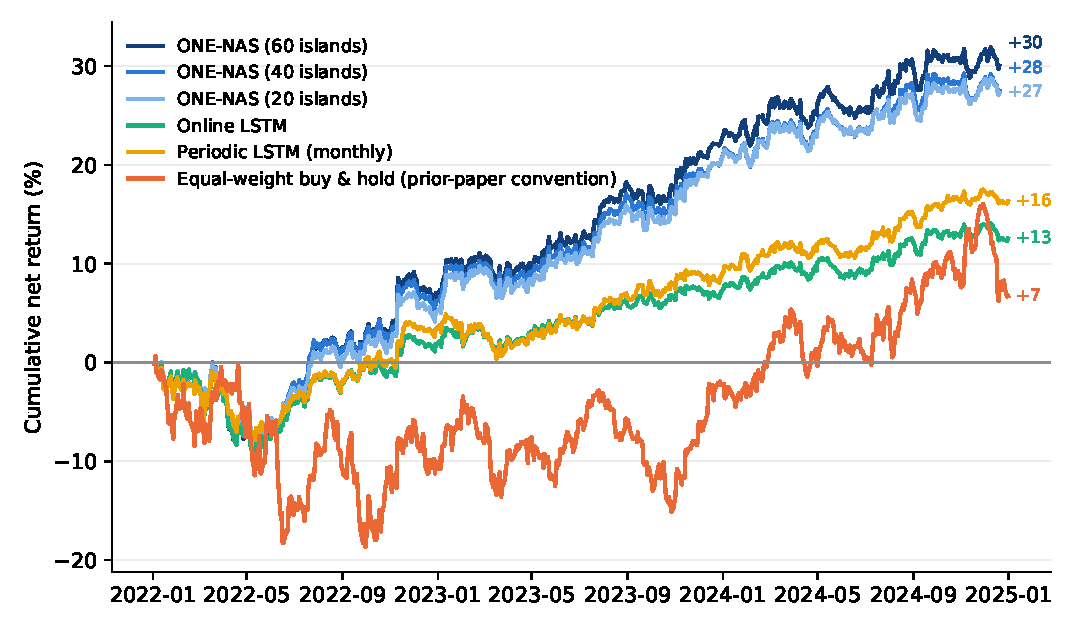
\includegraphics[width=0.92\textwidth]{net_curves.pdf}
\caption{Cumulative net return, 2022--2024 (books restarted at window
start). Buy-and-hold follows the prior-study benchmark convention.}
\label{fig:curves}
\end{figure*}

\begin{table}[t]
\centering
\footnotesize
\begin{tabular}{@{}lrr@{}}
\toprule
Comparison & $\Delta$net & paired $t$ \\
\midrule
vs.\ ONE-NAS (60 isl.)       & $-2.5$  & $-1.63$ \\
vs.\ ONE-NAS (20 isl.)       & $+0.2$  & $0.10$ \\
vs.\ Online LSTM             & $+16.2$ & $7.32$ \\
vs.\ Online GRU              & $+15.8$ & $6.59$ \\
vs.\ Periodic LSTM (monthly) & $+12.7$ & $6.66$ \\
vs.\ Online AR$^{a}$         & $+34.9$ & $2.22$ \\
\bottomrule
\end{tabular}
\par\smallskip
{\footnotesize
Comparisons are over all 40 (panel, seed) cells unless noted. Buy \& hold
trades once and is not seed-paired, so no paired test is reported against
it. $^{a}$Deterministic; one run per panel, so $n{=}4$.\par}
\caption{Paired significance for Table~\ref{tab:window}: within-cell
difference in net return (\%) between ONE-NAS (40 islands, sleeves book)
and each other arm, over the (panel, seed) cells the two arms share,
2022--2024.}
\label{tab:paired}
\end{table}

\begin{table}[t]
\centering
\footnotesize
\begin{tabular}{@{}l@{\hspace{3pt}}r@{\hspace{3pt}}r@{\hspace{3pt}}r@{\hspace{3pt}}r@{\hspace{3pt}}r@{}}
\toprule
Arm & $1\times$ & $2\times$ & $3\times$ & $5\times$ & B/E$^{a}$ \\
\midrule
ONE-NAS (60 isl.)   & $+30.1$ & $+27.2$ & $+24.4$ & $+18.8$ & $11.6\times$ \\
ONE-NAS (40 isl.)   & $+27.5$ & $+24.7$ & $+21.8$ & $+16.0$ & $10.6\times$ \\
ONE-NAS (20 isl.)   & $+27.4$ & $+24.4$ & $+21.5$ & $+15.6$ & $10.3\times$ \\
Periodic LSTM       & $+14.8$ & $+11.4$ & $+8.0$  & $+1.2$  & $5.4\times$ \\
Online GRU          & $+11.7$ & $+8.3$  & $+4.9$  & $-1.8$  & $4.5\times$ \\
Online LSTM         & $+11.3$ & $+8.1$  & $+4.9$  & $-1.5$  & $4.5\times$ \\
Online AR           & $-3.3$  & $-6.0$  & $-8.8$  & $-14.2$ & --- \\
\bottomrule
\end{tabular}
\par\smallskip
{\footnotesize
Scaling multiplies the realised per-name cost, so the cross-sectional
shape of costs is preserved and wide-spread names remain the expensive
ones. The $1\times$ column is the sleeves-book column of
Table~\ref{tab:window}. $^{a}$Break-even: the cost multiple at which net
return reaches zero.\par}
\caption{Cost sensitivity: net return (\%) on 2022--2024 as the realised
per-name transaction cost is scaled by the stated multiple. ONE-NAS
tolerates the harshest cost assumption of any arm.}
\label{tab:costs}
\end{table}

\begin{table*}[t]
\centering
\small
\begin{tabular}{@{}llrrrr@{}}
\toprule
Fleet & Window & Single & Ensemble & $\Delta$net ($t$) & $\Delta$Sharpe ($t$) \\
\midrule
60 isl.\ ($n{=}10$) & 2022--24 & $+1.0$ / $0.09$  & $+30.1$ / $0.93$ & $+29.1$ $(18.3)$ & $+0.84$ $(14.1)$ \\
40 isl.\ ($n{=}10$) & 2022--24 & $+4.5$ / $0.21$  & $+27.5$ / $0.87$ & $+23.0$ $(18.2)$ & $+0.66$ $(14.7)$ \\
20 isl.\ ($n{=}10$) & 2022--24 & $+4.7$ / $0.25$  & $+27.4$ / $0.87$ & $+22.6$ $(14.9)$ & $+0.62$ $(14.9)$ \\
\midrule
40 isl.\ ($n{=}5$)$^{a}$ & 2016--19 & $+8.9$ / $0.30$  & $+36.7$ / $1.22$ & $+27.8$ $(7.5)$  & $+0.92$ $(6.6)$ \\
\bottomrule
\end{tabular}
\par\smallskip
{\footnotesize $^{a}$Replication on the 2016--2019 tuning-span fleets.\par}
\caption{Prediction rule, within-run paired: single global-best genome
vs.\ island-champion rank-mean ensemble from the same runs (sleeves book).
Net \% / Sharpe; $\Delta$ = ensemble $-$ single, paired $t$ over seeds.}
\label{tab:m1}
\end{table*}

\begin{figure}[t]
\centering
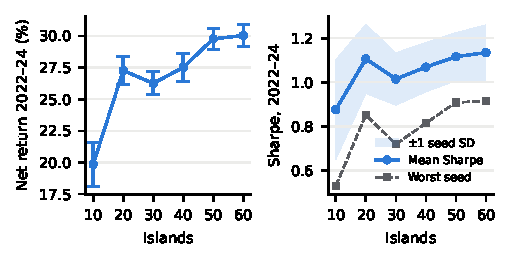
\includegraphics[width=\columnwidth]{islands_scaling.pdf}
\caption{Performance vs.\ island count (2022--2024, registered sleeves
book; 10 seeds $\times$ 4 panels at every width). Left: pooled net return
(mean $\pm$ SE). Right: Sharpe --- mean with $\pm$1 seed-SD band, and the
worst seed. Both rise steeply from 10 to about 20 islands ($+19.9 \to
+27.3$ net, Sharpe $0.88 \to 1.11$) and then flatten: across 20--60 the
cells span $+26$ to $+30$ net and Sharpe $1.01$--$1.13$, and are not
separable at this replication. Seed dispersion narrows over the same
range (SD $0.227 \to 0.11$--$0.13$; worst seed $0.53 \to 0.91$), so the
widest settings are the most reliable as well as the strongest, though
the improvement is not monotone width by width. The 40-island headline
was fixed on the 2016--2019 tuning span (Table~\ref{tab:tunewidth})
before this curve was measured, and the nominally higher 50- and
60-island cells are evaluation-span measurements that were tested on the
tuning span and found indistinguishable from 40.}
\label{fig:islands}
\end{figure}

\begin{table}[t]
\centering
\footnotesize
\begin{tabular}{@{}r@{\hspace{5pt}}r@{\hspace{5pt}}r@{\hspace{5pt}}r@{\hspace{5pt}}r@{\hspace{5pt}}r@{}}
\toprule
Islands & $n$ & rank IC & Net\% & Sharpe & MDD\% \\
\midrule
8  & 20 & $+0.0132$ & $+26.0$ & $0.92$ & $11.6$ \\
16 & 20 & $+0.0149$ & $+31.5$ & $1.11$ & $10.2$ \\
20 & 20 & $+0.0157$ & $+36.0$ & $1.24$ & $10.4$ \\
40 & 40 & $+0.0169$ & $+36.2$ & $1.21$ & $10.4$ \\
50 & 40 & $+0.0170$ & $+36.4$ & $1.21$ & $10.4$ \\
60 & 40 & $+0.0168$ & $+35.7$ & $1.19$ & $10.8$ \\
\bottomrule
\end{tabular}
\par\smallskip
{\footnotesize
$n$ is (panel, seed) cells; widths 8--20 were run at seeds 42--46 and
40--60 at 42--51. Restricting every width to the shared seeds 42--46
leaves the ordering unchanged.\par}
\caption{Island count on the tuning span, 2016--2019, registered sleeves
book. This is the span on which the width was chosen. Rank IC rises from
8 to about 20 islands and is flat above it: the 40-, 50- and 60-island
cells span $0.0168$--$0.0170$ and are not separable (paired against 40,
largest $|t|=0.23$). The 40-island headline therefore sits on the
plateau, while the 8-island setting of the original registration is
measurably below it.}
\label{tab:tunewidth}
\end{table}

\begin{table}[t]
\centering
\footnotesize
\begin{tabular}{@{}l@{\hspace{4pt}}r@{\hspace{4pt}}r@{\hspace{4pt}}r@{\hspace{4pt}}r@{}}
\toprule
Arm & bps/day & \%/yr & NW $t$ & Beta \\
\midrule
ONE-NAS (60 islands)     & $+4.43$ & $+11.2$ & $+2.73$ & $+0.120$ \\
ONE-NAS (40 islands)     & $+4.05$ & $+10.2$ & $+2.56$ & $+0.109$ \\
ONE-NAS (20 islands)     & $+3.99$ & $+10.0$ & $+2.77$ & $+0.114$ \\
Periodic LSTM (monthly)  & $+2.39$ & $+6.0$  & $+2.01$ & $+0.046$ \\
Online LSTM              & $+1.93$ & $+4.9$  & $+1.61$ & $+0.069$ \\
Online GRU               & $+1.75$ & $+4.4$  & $+1.91$ & $+0.033$ \\
Online AR                & $-0.81$ & $-2.1$  & $-0.64$ & $+0.045$ \\
\midrule
Buy \& hold              & $-0.91$ & $-2.3$  & $-0.72$ & $+0.802$ \\
\bottomrule
\end{tabular}
\caption{Factor-adjusted alphas: pooled daily book returns regressed on
the Fama--French three factors plus momentum, 2022--2024, Newey--West lag
10. All three ONE-NAS widths clear $|t|{>}2$; among the baselines only the
monthly-retrained LSTM does, at $t{=}2.01$.}
\label{tab:alphas}
\end{table}

\begin{table}[t]
\centering
\footnotesize
\begin{tabular}{@{}l@{\hspace{3pt}}c@{\hspace{3pt}}c@{\hspace{3pt}}c@{\hspace{3pt}}c@{\hspace{3pt}}c@{}}
\toprule
Fleet & $N$ & $\rho$ & Member & Ensemble & Predicted \\
\midrule
20 islands & 20 & 0.166 & $+0.0068$ & $+0.0145$ & $+0.0149$ \\
40 islands & 40 & 0.150 & $+0.0065$ & $+0.0153$ & $+0.0156$ \\
60 islands & 60 & 0.163 & $+0.0067$ & $+0.0157$ & $+0.0160$ \\
\bottomrule
\end{tabular}
\caption{Ensemble diversity mechanism: member rank IC, pairwise member
prediction correlation $\rho$, measured ensemble IC, and the
equicorrelated averaging prediction $m\sqrt{N/(1+(N-1)\rho)}$.}
\label{tab:diversity}
\end{table}

\begin{table}[t]
\centering
\small
\begin{tabular}{@{}lr@{\quad}lr@{}}
\toprule
Configuration & $\Delta$net & Configuration & $\Delta$net \\
\midrule
C0 (registered)      & $+3.9$  & NTS 600            & $+12.8$ \\
Select: IC-gated     & $+0.5$  & Rounds 2           & $+11.0$ \\
Select: IC           & $+2.8$  & PER $\alpha$ 0.4   & $+4.0$  \\
Target: 5-day CS     & $+4.5$  & PER $\alpha$ 0.8   & $+11.7$ \\
5-day CS + IC-gated  & $+1.8$  & PER $\lambda{\times}3$ & $+20.6$ \\
Elite 5 / gen 10     & $+9.6$  & BP epochs 20       & $+12.5$ \\
Elite 5 / gen 15     & $+11.1$ & Repop.\ 25         & $+7.0$  \\
Repop.\ 100          & $+9.6$  & PER off (uniform)  & $+9.3$  \\
\bottomrule
\end{tabular}
\par\smallskip
{\footnotesize Mean $+8.3$; $n{=}6$ runs per cell (2 panels $\times$ 3
seeds).\par}
\caption{Ensembling gain (ensemble $-$ single champion, within-run, net \%
on 2016--2019) inside every trained hyperparameter configuration; positive
in 16/16 cells.}
\label{tab:invariance}
\end{table}

\begin{table}[t]
\centering
\small
\begin{tabular}{@{}lr@{}}
\toprule
Population evolving online since 2020-01 & $+26.5$ \\
Cold start at 2022-01                     & $+12.3$ \\
\bottomrule
\end{tabular}
\caption{Online continuity: pooled net (\%) on 2022--2024, frozen 8-island
configuration.}
\label{tab:continuity}
\end{table}

\begin{table}[t]
\centering
\footnotesize
\begin{tabular}{@{}l@{\hspace{4pt}}l@{}}
\toprule
Hyperparameter & Value \\
\midrule
Islands & 40 (headline); 8 (reg.) \\
Elite population / island & 8 \\
Generated / island / generation & 5 \\
Repopulation frequency & every 50 gen. \\
Selection metric & validation MSE \\
Prediction rule & champion rank-mean \\
Target & 1-day CS rank-normal \\
Seq.\ len.\ / step / val.\ sets & 40 / 5 / 5 \\
Train subseq.\ / genome & 2000 \\
Backprop.\ epochs / genome & 10 \\
Replay (PER) $\alpha$, $\lambda$, $\epsilon$ & 0.6, 0.007, $10^{-8}$ \\
Rounds / generation & 1 \\
Node types & simple, UGRNN, MGU, \\
 & GRU, $\Delta$-RNN, LSTM \\
Mut.\ / intra- / inter-crossover & 0.7 / 0.2 / 0.1 \\
Warm-up generations & 50 \\
\bottomrule
\end{tabular}
\caption{ONE-NAS hyperparameter settings (selected on 2016--2019
validation data, disjoint from the evaluation span). Replay sampling
ablated: PER vs.\ uniform shows no advantage on the tuning objective
($\Delta$IC $-0.0024$, $t{=}-1.9$).}
\label{tab:hps}
\end{table}

\input{06-Conclusion}

\bibliography{99-References}

\appendix
% 80-Appendix.tex -- appendix material.
% Input from 00-main.tex AFTER \bibliography, preceded by
% \appendix so the section numbering restarts.

\section{Appendix}

\subsection{Configuration and Hyperparameter Search}

Table~\ref{tab:hps} lists the settings used for every ONE-NAS
run reported in the paper. Table~\ref{tab:hpscreen} gives the
per-cell outcome of the search that selected them.

\begin{table}[t]
\centering
\footnotesize
\begin{tabular}{@{}l@{\hspace{4pt}}l@{}}
\toprule
Hyperparameter & Value \\
\midrule
Islands & 40 (headline); 8 (reg.) \\
Elite population / island & 8 \\
Generated / island / generation & 5 \\
Repopulation frequency & every 50 gen. \\
Selection metric & validation MSE \\
Prediction rule & champion rank-mean \\
Target & 1-day CS rank-normal \\
Seq.\ len.\ / step / val.\ sets & 40 / 5 / 5 \\
Train subseq.\ / genome & 2000 \\
Backprop.\ epochs / genome & 10 \\
Replay (PER) $\alpha$, $\lambda$, $\epsilon$ & 0.6, 0.007, $10^{-8}$ \\
Rounds / generation & 1 \\
Node types & simple, UGRNN, MGU, \\
 & GRU, $\Delta$-RNN, LSTM \\
Mut.\ / intra- / inter-crossover & 0.7 / 0.2 / 0.1 \\
Warm-up generations & 50 \\
\bottomrule
\end{tabular}
\caption{ONE-NAS hyperparameter settings (selected on 2016--2019
validation data, disjoint from the evaluation span). Replay sampling
ablated: PER vs.\ uniform shows no advantage on the tuning objective
($\Delta$IC $-0.0024$, $t{=}-1.9$).}
\label{tab:hps}
\end{table}

% Generated by scripts/pooled/econ/hp_appendix_table.py from
% results_econ/hp_screen_score.csv; regenerate rather than editing.
% hp_screen_table.tex -- generated by scripts/pooled/econ/hp_appendix_table.py
\begin{table*}[t]
\centering
\footnotesize
\begin{tabular}{@{}l@{\hspace{2pt}}r@{\hspace{2pt}}r@{\hspace{2pt}}r@{\hspace{2pt}}r@{}}
\toprule
Configuration & rank IC & Net\% & Sharpe & $\Delta$IC ($t$) \\
\midrule
C0 (control) & $+0.0172$ & $+23.2$ & $0.81$ & --- \\
Selection: gated rank IC & $+0.0153$ & $+10.4$ & $0.26$ & $-0.0019$ (-0.5) \\
Selection: rank IC & $+0.0149$ & $-1.4$ & $-0.09$ & $-0.0023$ (-1.0) \\
Target: 5-day horizon & $+0.0150$ & $+31.3$ & $1.00$ & $-0.0022$ (-1.0) \\
Target 5-day + gated & $+0.0089$ & $+26.8$ & $0.76$ & $-0.0083$ (-4.4) \\
Elite 5 / generated 10 & $+0.0132$ & $+25.3$ & $0.94$ & $-0.0040$ (-2.0) \\
Elite 5 / generated 15 & $+0.0083$ & $+17.8$ & $0.67$ & $-0.0089$ (-1.9) \\
Repopulation every 25 & $+0.0151$ & $+19.8$ & $0.62$ & $-0.0021$ (-1.0) \\
Repopulation every 100 & $+0.0166$ & $+31.1$ & $1.05$ & $-0.0006$ (-0.4) \\
600 train subseq. & $+0.0164$ & $+26.5$ & $0.97$ & $-0.0008$ (-0.4) \\
2 generations / window & $+0.0152$ & $+30.1$ & $1.01$ & $-0.0020$ (-0.8) \\
Replay $\alpha=0.4$ & $+0.0160$ & $+30.9$ & $1.13$ & $-0.0012$ (-0.7) \\
Replay $\alpha=0.8$ & $+0.0149$ & $+27.7$ & $0.98$ & $-0.0023$ (-1.1) \\
Replay $\lambda=0.021$ & $+0.0149$ & $+33.2$ & $1.11$ & $-0.0023$ (-0.8) \\
Replay off (uniform) & $+0.0148$ & $+31.9$ & $1.15$ & $-0.0024$ (-1.4) \\
20 backprop.\ epochs & $+0.0188$ & $+35.1$ & $1.26$ & $+0.0016$ (0.8) \\
\bottomrule
\end{tabular}
\par\smallskip
{\footnotesize
All cells on the tuning span, 2016--2019, at $n{=}6$ runs each
(2 panels $\times$ 3 seeds). $\Delta$IC is paired against the
control on the cells the two share. Adoption required
$\Delta$IC $\ge +0.0020$ at $t \ge 2$; no cell met it, so the
control configuration is the one reported in the paper.\par}
\caption{Hyperparameter screen, every trained cell. Each varies
one axis from the control.}
\label{tab:hpscreen}
\end{table*}



% Check whether the conference requires a reproducibility checklist to be included in the paper.
% If so, you can uncomment the following line and ajust the path to include it.
% \input{ReproducibilityChecklist.tex}

\end{document}
